%\documentclass[mathserif]{beamer}
\documentclass[handout]{beamer}
%\usetheme{Goettingen}
\usetheme{Warsaw}
%\usetheme{Singapore}
%\usetheme{Frankfurt}
%\usetheme{Copenhagen}
%\usetheme{Szeged}
%\usetheme{Montpellier}
%\usetheme{CambridgeUS}
%\usecolortheme{}
%\setbeamercovered{transparent}
\usepackage[english, activeacute]{babel}
\usepackage[utf8]{inputenc}
\usepackage{amsmath, amssymb}
\usepackage{dsfont}
\usepackage{graphics}
\usepackage{cases}
\usepackage{graphicx}
\usepackage{pgf}
\usepackage{epsfig}
\usepackage{amssymb}
\usepackage{multirow}	
\usepackage{amstext}
\usepackage[ruled,vlined,lined]{algorithm2e}
\usepackage{amsmath}
\usepackage{epic}
\usepackage{epsfig}
\usepackage{fontenc}
\usepackage{framed,color}
\usepackage{palatino, url, multicol}
\usepackage{listings}
%\algsetup{indent=2em}


\vspace{-0.5cm}
\title{Directed Graphical Models}
\vspace{-0.5cm}
\author[Felipe Bravo Márquez]{\footnotesize
%\author{\footnotesize  
 \textcolor[rgb]{0.00,0.00,1.00}{Felipe José Bravo Márquez}} 
\date{ \today }




\begin{document}
\begin{frame}
\titlepage


\end{frame}


%%%%%%%%%%%%%%%%%%%%%%%%%%%


\begin{frame}{Directed Graphical Models}
\scriptsize{
\begin{itemize}
\item Probabilistic graphical models (PGMs) provide a visual representation of the underlying structure of a joint probablity distribution \cite{ruozzi}.


\item In this class we will focus on directed graphical models (DGMs), which are one type of PGM.

\item Directed graphical models (DGMs) are a family of probability distributions that admit a compact parametrization that can be naturally described using a \textbf{directed acyclic graph}.

\item DGMs were created by Turig prize awardee Judea Pearl under the name of \textbf{Bayesian networks}.

\item We won't use that term much in this class because statistical inference for DGMs can be performed using frequentist or Bayesian methods, which makes the name misleading \cite{wasserman2013all}.


 
\end{itemize}



} 

\end{frame}


\begin{frame}{Judea Pearl}

\begin{figure}[h!]
	\centering
	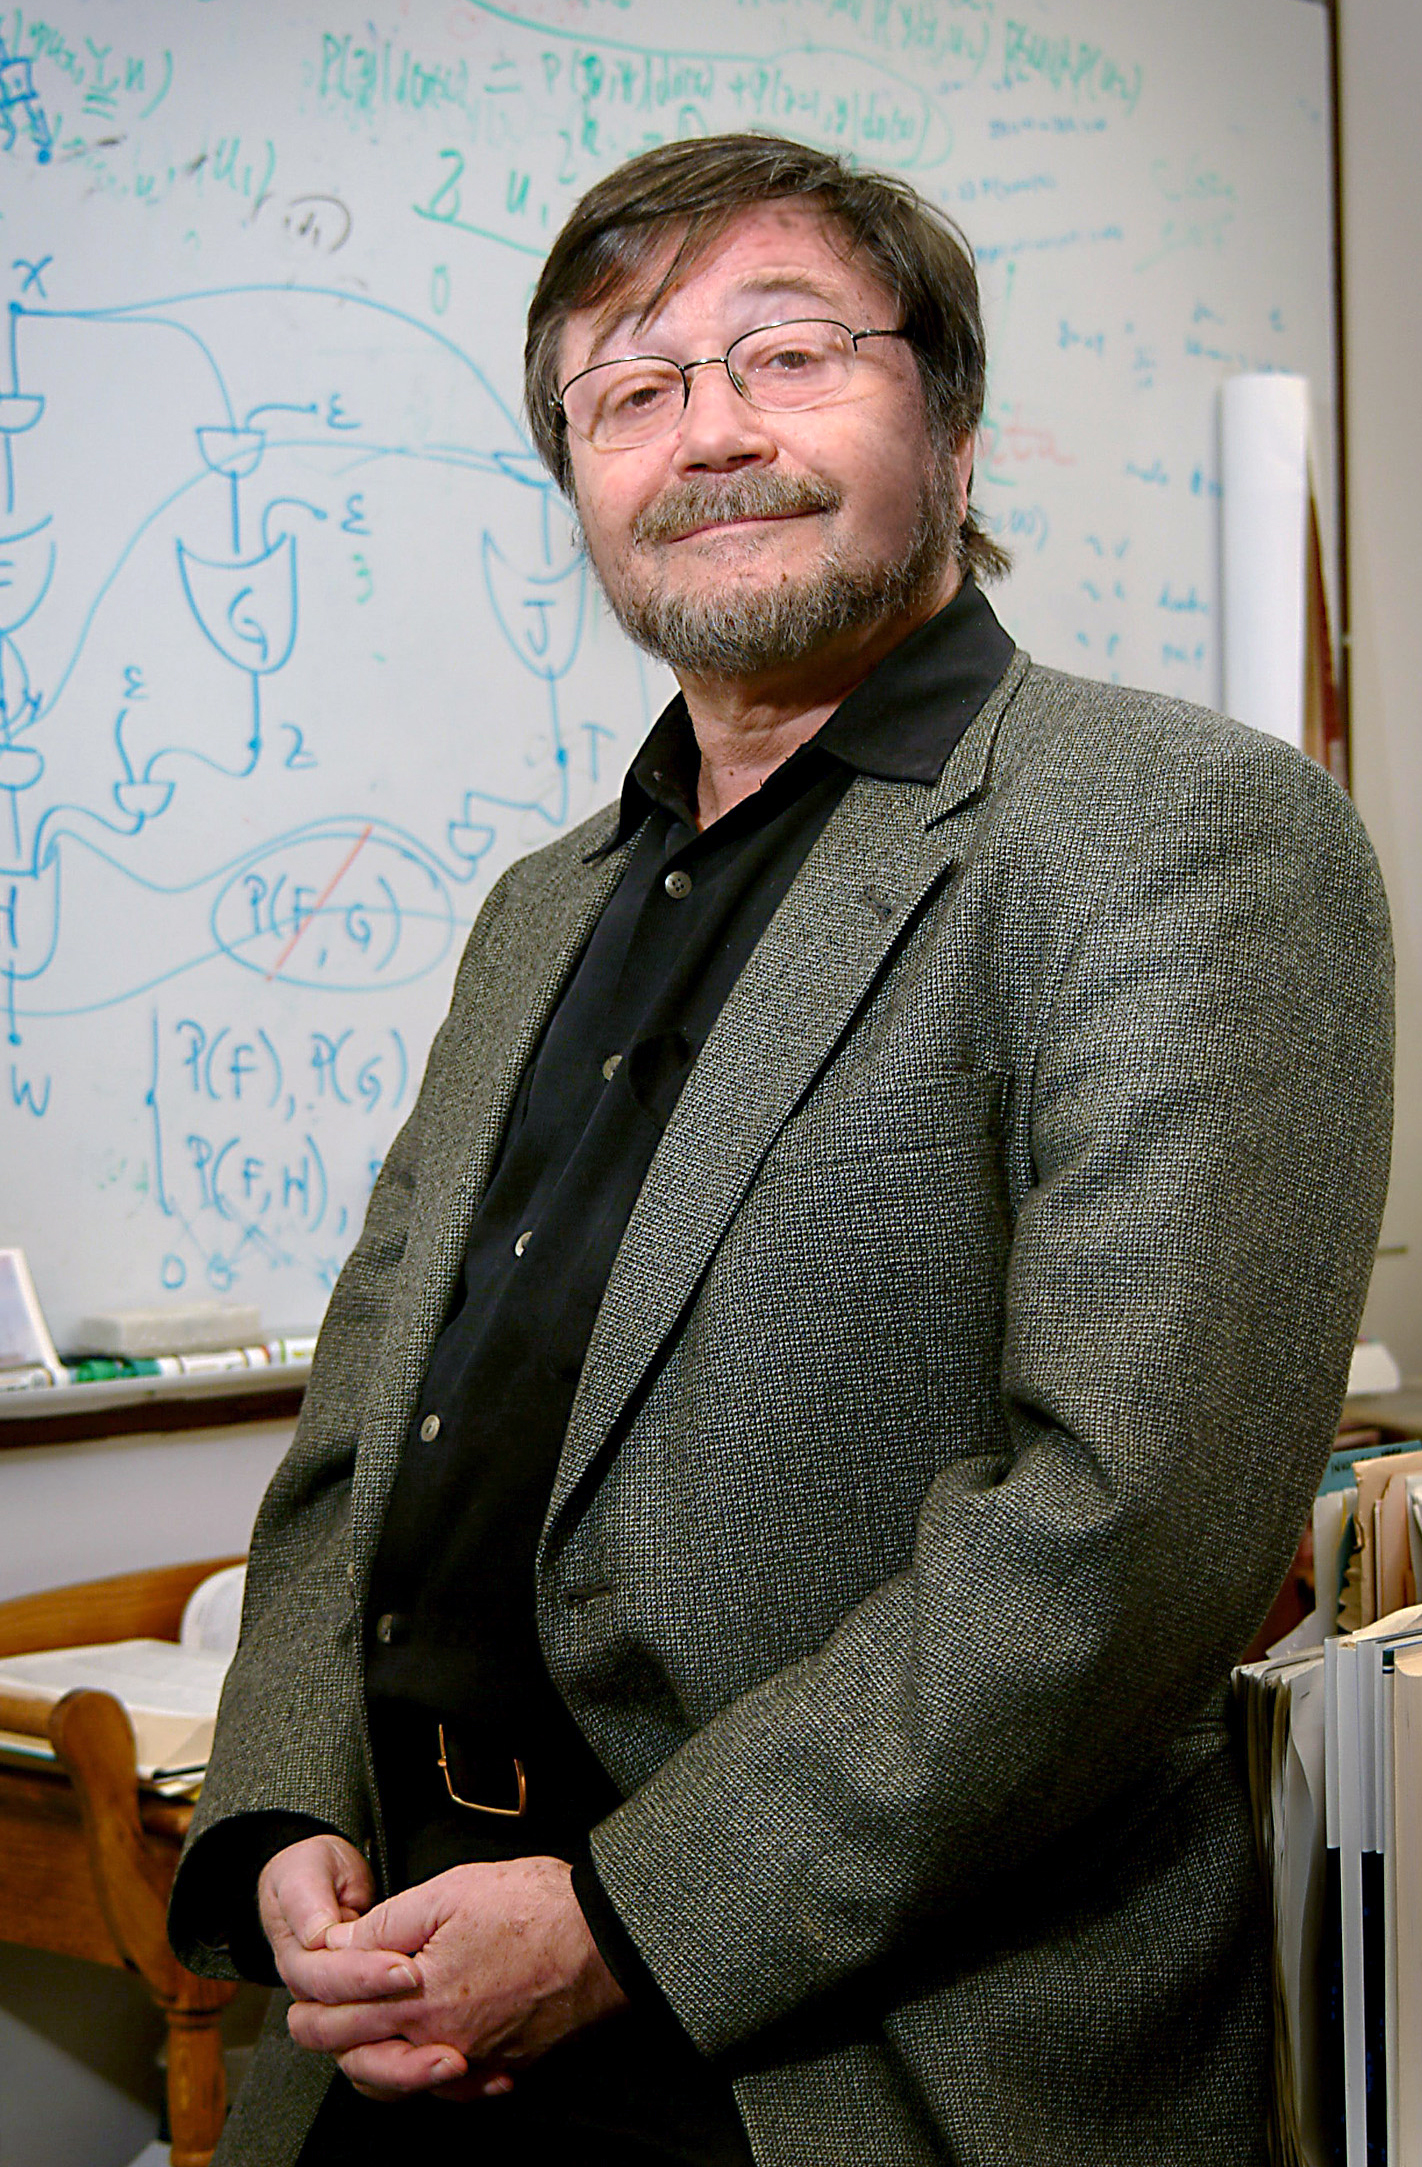
\includegraphics[scale=0.8]{pics/judea.jpg}
	\caption{Judea Pearl, source: \url{https://www.amacad.org/person/judea-pearl}}
	\end{figure} 


\end{frame}


\begin{frame}{Directed Graphical Models}
\scriptsize{
\begin{itemize}
\item DGMs link two very different branches of mathematics: probability and graph theory. 

\item They also have intriguing connections to philosophy, particularly the question of \textbf{causality}.

\item At the same time, they are widely used in statistics and machine learning.

\item DGMs can be used to solve problems in fields as diverse as medicine, language processing, vision, and many others \cite{ermon_kuleshov}. 

\item But before introducing them more formally we need to learn the following mathematical concepts:

\begin{enumerate}
\scriptsize{
 \item Conditional independence
 \item The chain rule of probability
 \item Directed acyclical graphs (DAGs) }
\end{enumerate}

 
\end{itemize}



} 

\end{frame}



\begin{frame}{Conditional Independence}
\scriptsize{
\begin{itemize}

\item Two random variables $X$ and $Y$ are independent, written $X \perp Y$ if $f(x,y)=f(x)f(y)$ for all values of $x$, $y$.


\item This also implies that $f(x|y)=f(x)$ and $f(y|x)=f(y)$.


\item Notice that $f$ can be either a density function for continous random variables or a probability mass function for discrete random variables.

\item In the same way  $f(x|y)$ and $f(y|x)$ correspond to conditional densities or mass functions. 

\item Now, suppose we have three random variables $A,B,C$. 

\item $A$ and $B$ are conditionally independent given $C$, written $A \perp B | C$, if:

\begin{displaymath}
f(a|b,c) = f(a|c)
\end{displaymath}


for all a, b and c.


 
\end{itemize}




} 

\end{frame}



\begin{frame}{Conditional Independence}
\scriptsize{

\begin{itemize}
 \item Intuitively, $A \perp B | C$ means that, once you know $C$, $B$ provides no extra information about $A$.

\item Notice that $A \perp B | C$ doesn't necessarily imply that $A \perp B$.
 
\end{itemize}



\begin{block}{Example}
\begin{itemize}
 \item Let $H,V,A$ be three random variables representing a person's height, vocabulary and age.
 \item H and V are dependent $f(v|h) \neq f(v)$ 
 since very small people tend to be children, known for their more basic vocabularies. 
 \item But knowing that two people are 19 years old (i.e., conditional on age) there is no reason to think that one person's vocabulary is larger if we are told that they are taller: 
 \begin{displaymath}
 f(v|h,a)=f(v|a) \Leftrightarrow V \perp H | A 
 \end{displaymath}

\end{itemize}


\end{block}





} 

\end{frame}


\begin{frame}{The chain rule of probability}
\scriptsize{
\begin{itemize}

\item For a set of random variables $X_1,\dots, X_n$, the chain rule of probability allow us to express the joint probability function $f(x_1,x_2,\dots, x_n)$ as a product of $n$ conditional probabilities:



\begin{displaymath}
f(x_1,x_2,\dots,x_n)=f(x_1)f(x_2|x_1)f(x_3|x_2,x_1)\dots f(x_n|x_{n-1},\dots,x_2,x_1).
 \end{displaymath}

\item For example for the case of $n=3$

\begin{displaymath}
f(x_1,x_2,x_3)=f(x_1)f(x_2|x_1)f(x_3|x_2,x_1)
 \end{displaymath}

using the definition of conditional probabilities we have that


\begin{displaymath}
 f(x_2|x_1) = f(x_1,x_2)/f(x_1)
\end{displaymath}

 and \begin{displaymath}
f(x_3|x_2,x_1)=f(x_1,x_2,x_3)/f(x_1,x_2)       
     \end{displaymath}

\item By replacing these expressions into the chain of products, many expressions cancel out and we obtain $f(x_1,x_2,x_3)$.     

\end{itemize}



} 

\end{frame}


\begin{frame}{Joint Probabilities}
\scriptsize{
\begin{itemize}

\item Expressing a joint probability function can be expensive.

\item For example if there are $m$ binary random variables, the complete distribution is specificied by $2^{m}-1$ joint probabilities.

\item For example, if we have two Boolean variables $(A,B)$, we need the probabilities $\mathbb{P}(A,B)$, $\mathbb{P}(\neg A,B)$, $\mathbb{P}(A,\neg B)$, and $\mathbb{P}(\neg A, \neg B)$.

\item A joint distribution for a set of random variables gives all the information there is about the distribution.


\item Note that for $m$ boolean variables, the joint distribution contains $2^m$ values. 

\item However, the sum of all the joint probabilities must be 1 because the probability of all possible outcomes must be 1. 

\item Thus, to specify the joint distribution, one needs to specify $2^{m-1}$ numbers.


\end{itemize}



} 

\end{frame}


\begin{frame}{Joint Probabilities}
\scriptsize{
\begin{itemize}



\item The main idea of DGMs is that by assuming that some variables are conditionally independent we can use the probability chain rule to represent the joint distribution more compactly.

\item For example in the previous example, a conditional independence assumption could be: $X_3 \perp X_2| X_1$: $f(x_3|x_2,x_1)= f(x_3|x_2)$.

\item Then our joint distribution would be reduced to:

\begin{displaymath}
f(x_1,x_2,x_3)=f(x_1)f(x_2|x_1)f(x_3|x_2)
 \end{displaymath}

 
\item In the following slides we will clarify these concepts with the Student example given in \cite{koller2009probabilistic}. 

\end{itemize}



} 

\end{frame}

\begin{frame}{The Student Example}
\scriptsize{
\begin{itemize}


\item Consider the problem faced by a company trying to hire a recent college graduate. 
\item The company's goal is to hire intelligent employees, but there is no way to test intelligence directly. 

\item However, the company has access to the student's SAT scores\footnote{The SAT is a standardized test widely used for college admissions in the United States.}, which are informative but not fully indicative. 

\item Thus, our probability space is induced by the two random variables Intelligence (I) and SAT (S). 
\item For simplicity, we assume that each of these takes two values: $Val(I) = \{i_1 , i_0 \}$, which represent
the values high intelligence ($i_1$ ) and low intelligence $(i_0)$.


\end{itemize}



} 

\end{frame}


\begin{frame}{The Student Example}
\scriptsize{
\begin{itemize}

\item Similarly $Val(S) = \{s_1 , s_0 \}$, which
also represent the values high (score) and low (score), respectively.

\item Thus, our joint probability function in this case has four entries. 
\item For example, one possible joint probability function $f$ would be:

\begin{table}
\centering
  \begin{tabular}{cc|c} \hline
$I$ & $S$ & $f(i,s)$  \\ \hline
$i^0$ & $s^0$ & 0.665 \\
$i^0$ & $s^1$ & 0.035 \\
$i^1$ & $s^0$ & 0.06 \\
$i^1$ & $s^1$ & 0.24 
\end{tabular} 
\end{table}

\item Notice that we would need 3 parameters to specify this joint probability function ($2^{m-1}$).

\item Alternatively, we could use the the chain rule of conditional probabilities to represent the joint probability function as follows:

\begin{displaymath}
 f(i,s) = f(i)f(s|i)
\end{displaymath}

\end{itemize}



} 

\end{frame}


\begin{frame}{The Student Example}
\scriptsize{
\begin{itemize}

\item Other factorizations obtained by changing the order of the variables are also valid (e.g., $f(i,s) = f(s)f(i|s)$).


\item However, it is convenient to represent the process in a way that is more compatible with causality.

\item Various factors (e.g., genetics, upbringing) first determined (stochastically) the student's intelligence.
\item Her/his performance on the SAT is determined (stochastically) by her/his  intelligence. 
\item We note that the models we construct are not required to follow causal intuitions, but they often do.



\end{itemize}



} 

\end{frame}


\begin{frame}{The Student Example}
\scriptsize{
\begin{itemize}

\item From a mathematical perspective, $ f(i,s) = f(i)f(s|i)$ leads to an alternative way of representing the joint probability function. 

\item Instead of specifying the various joint entries $f(i,s)$, we would specify it in the form of $f(i)$ and $f(s|i)$. 
\item Thus, we could represent the joint probability function using two tables.

\item The first one representing the marginal probability function of $I$.


\begin{table}
\centering
  \begin{tabular}{cc} \hline
$i^0$ & $i^1$  \\ \hline
0.7 & 0.3   
\end{tabular} 
\end{table}

\item These numbers can be easily verified from the previous table. For example 

\begin{displaymath}
f(i^{0})=f(i^{0},s^0)+f(i^{0},s^1)=0.665+0.035=0.7 
\end{displaymath}




\end{itemize}



} 

\end{frame}


\begin{frame}{The Student Example}
\scriptsize{
\begin{itemize}

\item The second table represents the conditional probability function of $S$ given $I$:

\begin{table}
\centering
  \begin{tabular}{c||cc} \hline
$I$ & $s^0$ & $s^1$  \\ \hline
$i^0$ & 0.95 & 0.05 \\
$i^1$ & 0.2 & 0.8 \\

\end{tabular} 
\end{table}

\item which can also be verified from previous table using the Bayes theorem. For example:

\begin{displaymath}
f(s^{0}|i^0)=f(s^{0},i^0)/f(i^0)= 0.665/0.7=0.95
\end{displaymath}

\item The conditional probability function $f(s| i)$ represents the probability that the student will succeed on his SATs in the two possible cases:
\begin{enumerate}
\scriptsize{
\item The case where the student's intelligence is low.
\item The case where it is high. }
\end{enumerate}


\end{itemize}



} 

\end{frame}


\begin{frame}{The Student Example}
\scriptsize{
\begin{itemize}

\item The conditional probability function asserts that a student of low intelligence is extremely unlikely to get a high SAT score ($f(s_1 | i_0 ) = 0.05$).
\item On the other hand, a student of high intelligence is likely, but far from
certain, to get a high SAT score ($f(s_1 | i_1 ) = 0.8$).

\item It is instructive to consider how we could parameterize this alternative representation. 
\item Here, we are using three Bernoulli distributions, one for $f(i)$, and two for $f(s | i_0)$ and $f(s|i_1)$.
\item Hence, we can parameterize this representation using three independent parameters, say $\theta_{i^1}$ ,$\theta_{s^1|i^1}$, and $\theta_{s^1|i^0}$

\item Recall that the original representation also required 3 parameters.



\end{itemize}



} 

\end{frame}


\begin{frame}{The Student Example}
\scriptsize{
\begin{itemize}

\item Thus, although the conditional representation is more natural
than the explicit representation of the joint, it is not more compact.

\item However, as we will soon see, the conditional parameterization provides a basis for our compact representations of more complex distributions.


\item Although we haven't defined directed acyclical graphs (DAGs) yet, it is instructive to see how this example would be represented as one. 

\begin{figure}[h!]
	\centering
	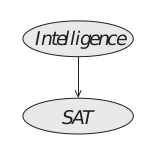
\includegraphics[scale=0.6]{pics/sat1.png}
	\end{figure} 


\item The DAG from above has a node for each of the two random variables $I$ and $S$, with an edge from $I$ to $S$ representing the direction of the dependence in this model.


\end{itemize}



} 

\end{frame}


\begin{frame}{The Student Example}
\scriptsize{
\begin{itemize}

\item Let's assume now that the company also has access to the student's grade $G$ in some course. 
\item In this case, our probability space is the joint probability function over the
three relevant random variables $I$, $S$, and $G$. 

\item We will assume that $I$ and $S$ are as before, and that $G$ takes on three values $g^1, g^2, g^3$, representing the grades A, B, and C, respectively.

\item So, the joint probability function  has twelve entries.

\item We can see that for any reasonable joint probability function  $f$, there are no independencies that hold.
\item The student's intelligence is clearly correlated both with SAT score and  grade.


\end{itemize}



} 

\end{frame}


\begin{frame}{The Student Example}
\scriptsize{
\begin{itemize}

\item The SAT score and grade are also not independent.
\item A high SAT score increases the chances of getting a high grade.

\item Thus, we may assume that, for our particular probability function  $f$,
$f(g^1|s^1) > f(g^1|s^0)$.

\item However, it is quite plausible that our probability function $f$ in this case satisfies a conditional independence property.

\item If we know that the student has high intelligence, a high grade on the SAT no longer gives us information about the student's performance in the class.

\item More formally: $f(g|s,i)=f(g|i)$ or $G \perp S|I$

\item So the joint probability function  can be reduced from

\begin{displaymath}
 f(i,s,g)=f(i)f(s|i)f(g|i,s)
\end{displaymath}

to

\begin{displaymath}
 f(i,s,g)=f(i)f(s|i)f(g|i) 
\end{displaymath}


\end{itemize}



} 

\end{frame}

\begin{frame}{The Student Example}
\scriptsize{
\begin{itemize}

\item Now our joint probability function  is specified by $f(i)$, $f(s|i)$, and $f(g|i)$.

\item While  $f(i)$, $f(s|i)$ might be the same as before, and  $f(g|i)$ might be:


\begin{table}
\centering
  \begin{tabular}{c||ccc} \hline
$I$ & $g^1$ & $g^2$ & $g^3$  \\ \hline
$i^0$ & 0.2 & 0.34 & 0.46 \\
$i^1$ & 0.74 & 0.17 & 0.09 \\

\end{tabular} 
\end{table}

\item Now we can calculate the joint probability of any combination of inputs.

\item For example: 

 \begin{align}
  f(i^1,s^1,g^2) & = f(i^1)f(s^1|i^1)f(g^2|i^1) \\
   & = 0.3*0.8*0.17 \\
   & = 0.0408
 \end{align}

\end{itemize}



} 

\end{frame}


\begin{frame}{The Student Example}
\scriptsize{
\begin{itemize}

\item The corresponding DAG would be as follows:


\begin{figure}[h!]
	\centering
	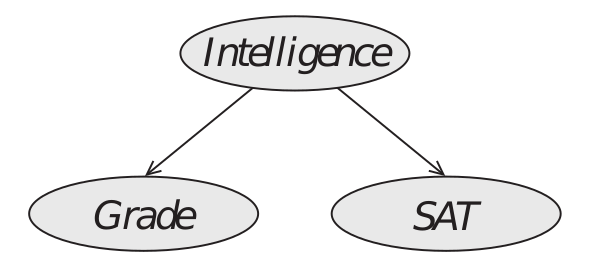
\includegraphics[scale=0.3]{pics/sat2.png}
	\end{figure} 

	\item In this case, the alternative parameterization is more compact than the joint. 
	\item We now have three Bernoulli distributions $f(i), f(s | i^1)$ and $f(s | i^0)$, and two three-valued categorical distributions $f(g | i_1 )$ and $f(g | i^0)$.
	\item A categorical distribution is  discrete probability distribution that describes the possible results of a random variable that can take on one of K possible categories, with the probability of each category separately specified\footnote{\url{https://en.wikipedia.org/wiki/Categorical_distribution}}.

	
\end{itemize}



} 

\end{frame}

\begin{frame}{The Student Example}
\scriptsize{
\begin{itemize}
	\item Each of the Bernoullis requires one independent parameter, and each three-valued categorical requires two independent parameters, for a total of seven. 
	\item By contrast, our joint probability function  has twelve entries, so that eleven independent parameters are required to specify an arbitrary joint probability function over these three variables.
\item It is important to note another advantage of this way of representing the joint: modularity.
\item When we added the new variable $G$, the joint probability function changed entirely. 
\item Had we used the explicit representation of the joint, we would have had to write down twelve new numbers. 
\item In the factored representation, we could reuse our local probability models for the variables $I$ and $S$, and specify only the probability model for $G$, the conditional probability function  $f(G | I)$. 
\item This property will turn out to be invaluable in modeling real-world systems.
	

\end{itemize}



} 

\end{frame}

\begin{frame}{Directed Acyclic Graphs (DAGs)}
\scriptsize{
\begin{itemize}

\item We just learned how the chain rule of probability and conditional independence assumptions enable us to obtain a compact representation of a joint probability function.

\item Now we are in a position to introduce DAGs.

\item A directed graph consists of a set of nodes with arrows between some nodes.



\item More formally, a directed graph G consists of a set of vertices V and an edge set E of ordered pairs of vertices.


\item If $(Y, X) \in E$  then there is an arrow pointing from Y to X. 

\begin{figure}[h!]
	\centering
	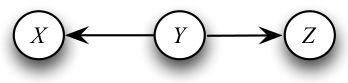
\includegraphics[scale=0.5]{pics/dag1.png}
	\caption{A directed graph with vertices $V = \{X, Y, Z\}$ and edges $E = \{(Y, X), (Y, Z)\}$.}
	\end{figure} 


 
\end{itemize}



} 

\end{frame}



\begin{frame}{Directed Acyclic Graphs (DAGs)}
\scriptsize{
\begin{itemize}
\item If an arrow connects two variables X and Y (in either direction) we say that X and Y are \textbf{adjacent}.


\item If there is an arrow from X to Y then X is a \textbf{parent} of Y and Y is a \textbf{child} of X.

\item The set of all parents of X is denoted by $\pi_{X}$ or $\pi(X)$.

\item A \textbf{directed path} between two variables is a set of arrows all pointing in the same direction linking one variable to the other such as the chain shown below:

\begin{figure}[h!]
	\centering
	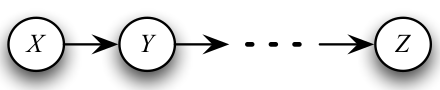
\includegraphics[scale=0.5]{pics/dag2.png}
	\caption{A chain graph with a directed path.}
	\end{figure} 

\item A sequence of adjacent vertices starting with X and ending with Y but ignoring the
direction of the arrows is called an \textbf{undirected path}.
	
\item X is an \textbf{ancestor} of Y if there is a directed path from X to Y (or X = Y ).

\item We also say that Y is a \textbf{descendant} of X.
 
\end{itemize}



} 

\end{frame}

\begin{frame}{Directed Acyclic Graphs (DAGs)}
\scriptsize{
\begin{itemize}
\item A directed path that starts and ends at the same variable is called a cycle.

\item A directed graph is acyclic if it has no cycles. 

\item In this case we say that the graph is a directed
acyclic graph or DAG. 


\begin{figure}[h!]
	\centering
	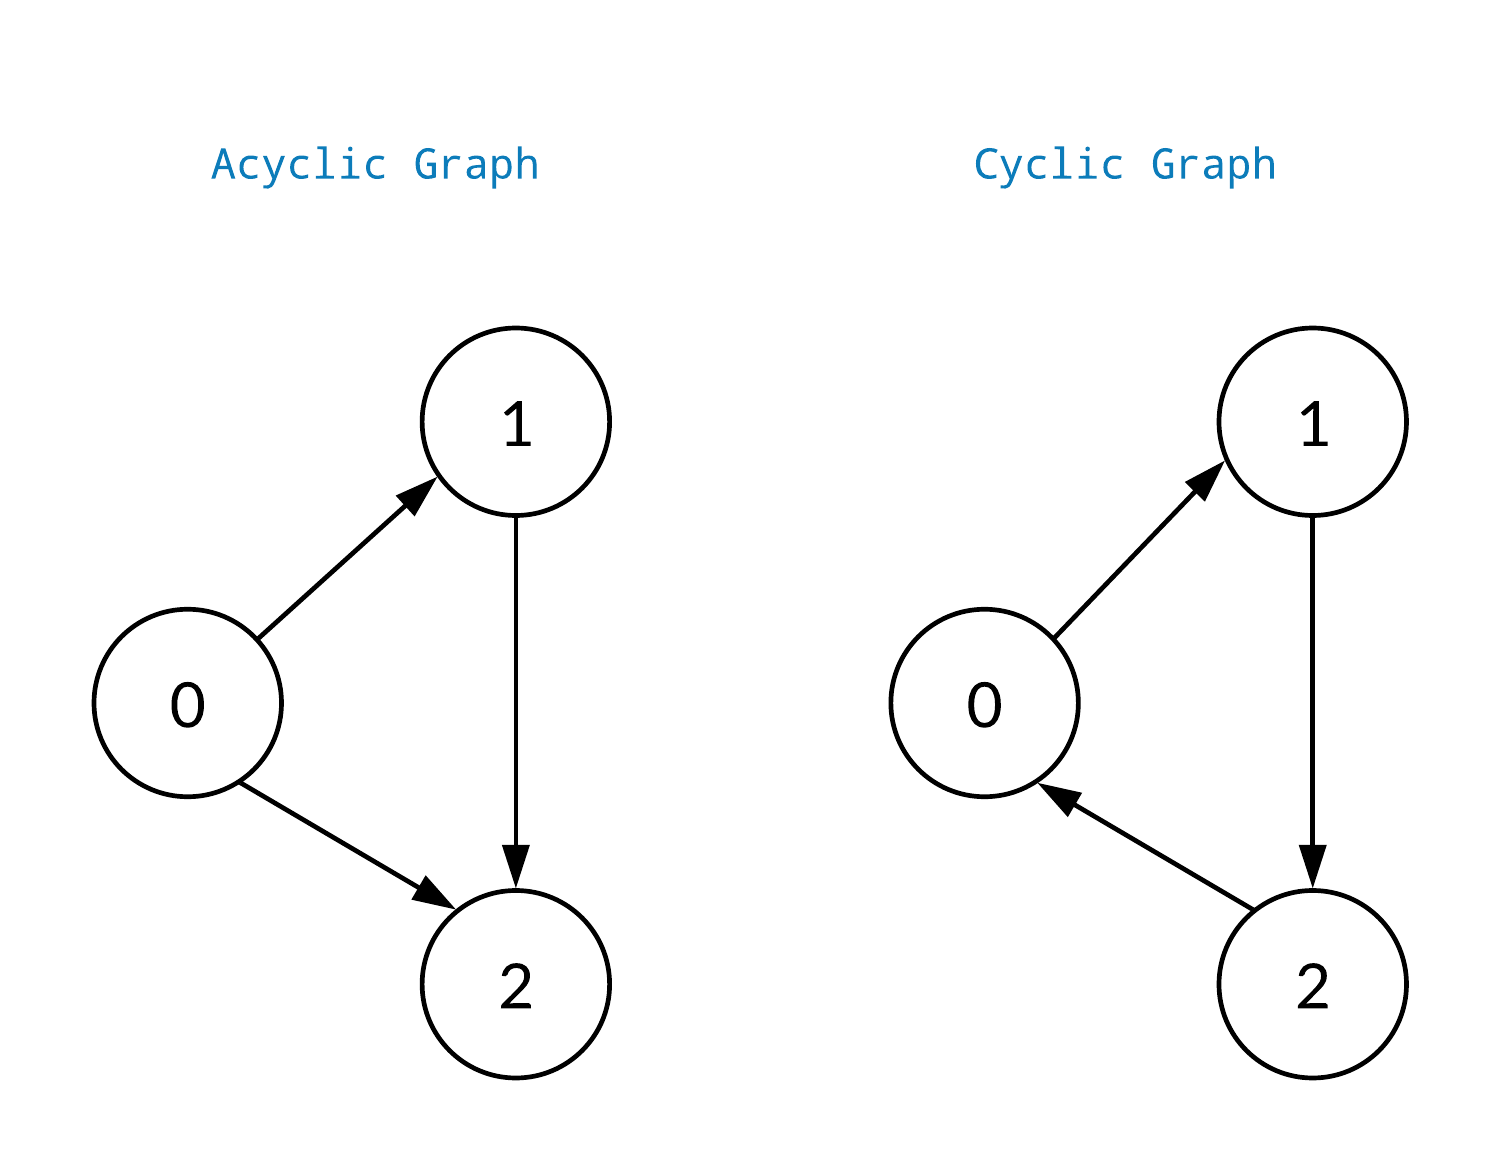
\includegraphics[scale=0.12]{pics/cycle.png}
	\end{figure} 



\item From now on, we only deal with directed acyclic graphs since it is very difficult to provide a coherent probability semantics over graphs with directed cycles.
 
 
 
\end{itemize}



} 

\end{frame}


\begin{frame}{Probability and DAGs}
\scriptsize{
\begin{itemize}

\item When a DAG is used to encode a joint probability function $f$ (density or mass) with given conditional independence relations, we have a Directed Graphical Model or Bayesian Network.

\item Warning: It is common to find terms DAG, DGM or Bayesian network used interchangeably in the literature. 


\item Let $G$ be a DAG with vertices $V = (X_1 , \dots , X_i, \dots, X_m )$. 
\item Each vertex $X_i$ is random variable


\item The edges of $G$ represent (conditional) independence relations between variables.



\item The order of vertices $(1,\dots,i,\dots,m)$ forms a topological sort on the random variables.

\item This means that every variable comes before all its descendants in the graph.





\end{itemize}



} 

\end{frame}

\begin{frame}{Probability and DAGs}
\scriptsize{
\begin{itemize}




\item For example, the next figure shows a DAG with four variables, the numbers indicate the topological order.

\begin{figure}[h!]
	\centering
	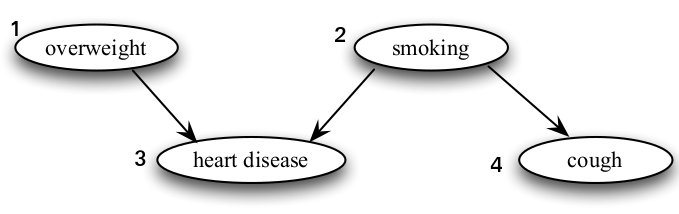
\includegraphics[scale=0.4]{pics/dag3.png}
	\end{figure} 

\item It is clear from the figure, that no vertex comes before any of its descendant in the DAG.	

\item Let $f$ be probability function  for $V$, $f(x_1,\dots,x_d)$,  we say that $G$ represents $f$, if

\begin{equation}
 f(x) = \prod_{j=1}^d f(x_j| \pi_{x_j}) 
\end{equation}



where $\pi_{x_j}$ is the set of parent nodes of $X_j$	
	


\end{itemize}



} 

\end{frame}


\begin{frame}{Probability and DAGs}
\scriptsize{
\begin{itemize}



\item Based on the equation above, probability function $f$ of the previous graph takes the following decomposition:

\begin{displaymath}
f(o,s,h,c) = f(o)f(s)f(h|o,s)f(c|s).  
\end{displaymath}



\item If no conditional independence assumptions were made, the joint probability function $f$ would the following:

\begin{displaymath}
f(o,s,h,c) = f(o)f(s|o)f(h|o,s)f(c|o,s,h)
\end{displaymath}

\item That means that the graph above encodes the following independence asssumptions:

\begin{enumerate}
 \item $f(s|o) = f(s)$ 
 \item $f(c|o,s,h) = f(c|s)$   
\end{enumerate}



\end{itemize}



} 

\end{frame}


\begin{frame}{Probability and DAGs}
\scriptsize{
\begin{itemize}



\item How can we know all the independence assumptions encoded by a DAG?

\item The answer is \textbf{d-separation}.


\item D-separation is a criterion for deciding,  whether a set X of variables is independent of another set Y, given a third set Z. 

\item The idea is to associate ``dependence'' with ``connectedness'' (i.e., the existence of a connecting path) and ``independence'' with ``unconnectedness'' or ``separation''.

\item Warning: D-separation is hard to understand.

\item Before trying to understand it we are going to introduce an R library for playing with DAGs: \textbf{Dagitty}.

\end{itemize}



} 

\end{frame}


\begin{frame}{Dagitty}
\scriptsize{
\begin{itemize}



\item DAGitty is a browser-based environment for creating, editing, and analyzing DAGs: \url{http://dagitty.net/}.

\begin{figure}[h!]
	\centering
	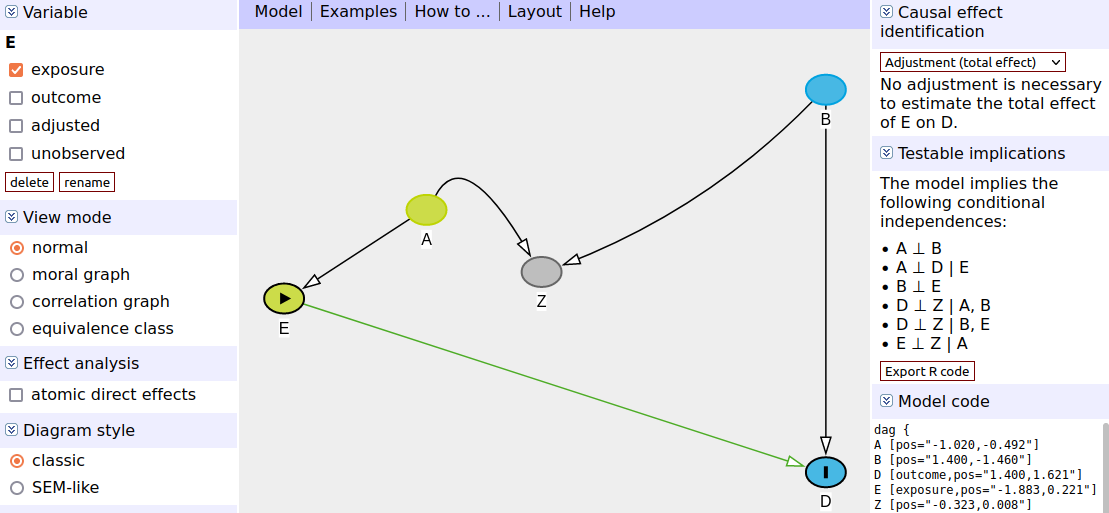
\includegraphics[scale=0.2]{pics/DAGitty.png}
	\end{figure} 



\item The R package ‘dagitty’ provides access to all of the capabilities of the DAGitty web application within R.


\end{itemize}





} 

\end{frame}



\begin{frame}[fragile]{Dagitty}
\scriptsize{
\begin{itemize}



\item We can use Dagitty to create the DAG from before with the command ``dag'':

\begin{verbatim}
> library(dagitty)
> 
> over <- dagitty("dag{ o -> h; s -> h; s ->c }")
\end{verbatim}


\item Now, in order to visualize the DAG we need to specify the coordinates of each vertex:

\begin{verbatim}
> coordinates(over) <- 
list( x=c(o=0,h=1,s=2,c=3) , y=c(o=0,h=1,s=0,c=1) )
> plot(over)  
\end{verbatim}

\begin{figure}[h!]
	\centering
	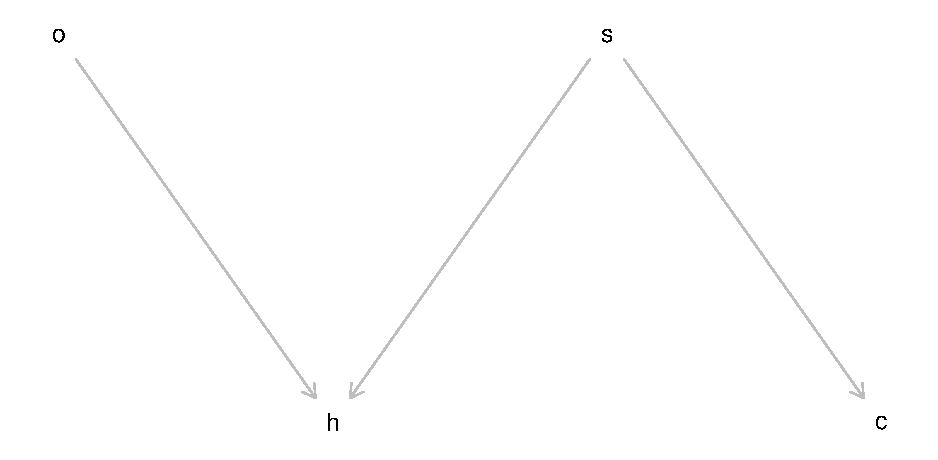
\includegraphics[scale=0.4]{pics/overdag1.pdf}
	\end{figure} 



\end{itemize}





} 

\end{frame}


\begin{frame}[fragile]{Dagitty}
\scriptsize{
\begin{itemize}



\item We can obtain the children of a node:

\begin{verbatim}
> children(over,"s")
[1] "c" "h"
\end{verbatim}

\item Or the parents:

\begin{verbatim}
> children(over,"s")
[1] "c" "h" 
\end{verbatim}


\item Or the undirected paths between two nodes:

\begin{verbatim}
> paths( over, "o", "c" )$path
[1] "o -> h <- s -> c"
\end{verbatim}

\item Or just the directed paths between two nodes:

\begin{verbatim}
> paths( over, "s", "c",directed = T )$path
[1] "s -> c" 
\end{verbatim}

\item Finally, we can obtain all the conditional independencies encoded by the DAG:

\begin{verbatim}
> impliedConditionalIndependencies(over)
c _||_ h | s
c _||_ o
o _||_ s 
\end{verbatim}


\end{itemize}


} 

\end{frame}

\begin{frame}{The Family Out Problem}
\scriptsize{
\begin{itemize}
\item We are going to use the ``family out'' example proposed by Eugene Charniak in  \cite{charniak1991bayesian} to understand d-separation.

\item The situation is as follows:

\item When Eugene goes home at night, he wants to know if his family is home before trying the doors. 

\item Often when his wife leaves the house, she turns on an outdoor light. 

\item Eugene's wife can also turn on the outdoor light if she is expecting a guest.

\item Also, they have a female dog. 

\item When nobody is home, the dog is put in the back yard. 

\item The same is true if the dog has bowel troubles. 

\item Finally, if the dog is in the backyard, Eugene's will probably hear her barking.

 
\end{itemize}



} 

\end{frame}



\begin{frame}{The Family Out Problem}
\scriptsize{
\begin{itemize}



\item All these causal relationships are represented in the DAG below:

 
 \begin{figure}[h!]
	\centering
	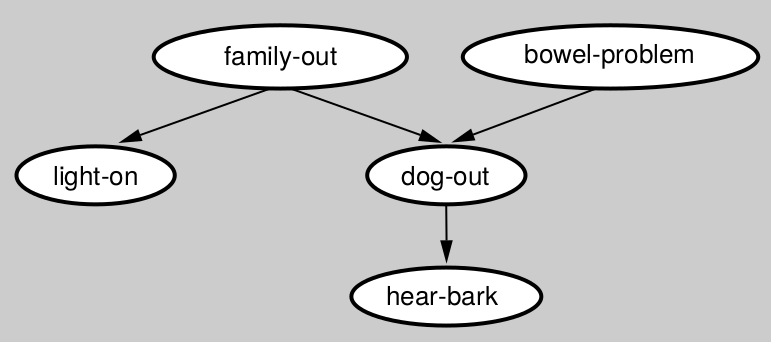
\includegraphics[scale=0.5]{pics/fodag.png}
	\end{figure} 
 
\item The numbers show the corresponding  position of each vertex in the topological sort. 
 
\item So, the joint probability function would be as follows:

\begin{displaymath}
 f(fo,bp,lo,do,hb)=f(fo)f(bp)f(lo|fo)f(do|fo,bp)f(hb|do)
\end{displaymath}



\end{itemize}



} 

\end{frame}


\begin{frame}{The Family Out Problem}
\scriptsize{



\begin{itemize}
\item Taking each random variable as binary, the marginal and conditional probability functions representing our DAG are shown below: 


 \begin{figure}[h!]
	\centering
	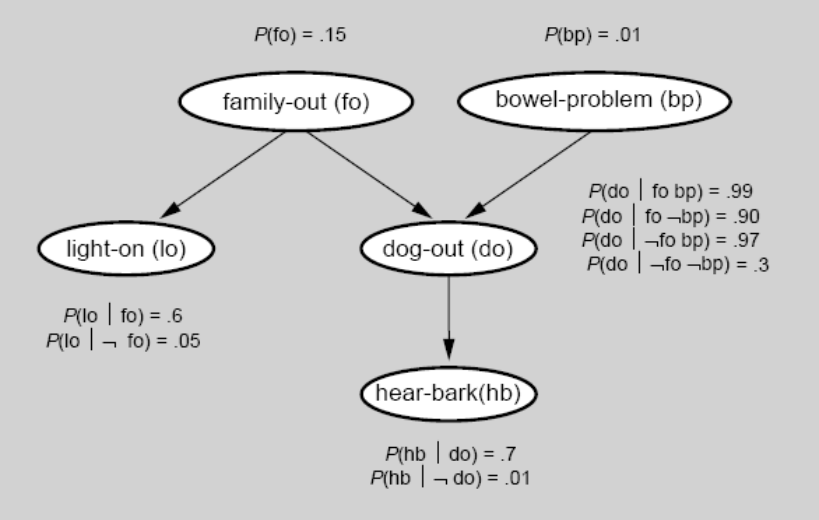
\includegraphics[scale=0.4]{pics/fodagProb.png}
	\end{figure} 






 
\end{itemize}



} 

\end{frame}


\begin{frame}[fragile]{The Family Out Problem}
\scriptsize{



\begin{itemize}
\item Let's build the DAG using dagitty:

\begin{verbatim}
fo <- dagitty("dag{ fo -> lo; fo -> do; bp -> do;do->hb }")
coordinates(fo) <- list( x=c(lo=0,fo=1,do=2,hb=2,bp=3)
                         , y=c(fo=0,bp=0,lo=1,do=1,hb=2) )
plot(fo) 
\end{verbatim}

 \begin{figure}[h!]
	\centering
	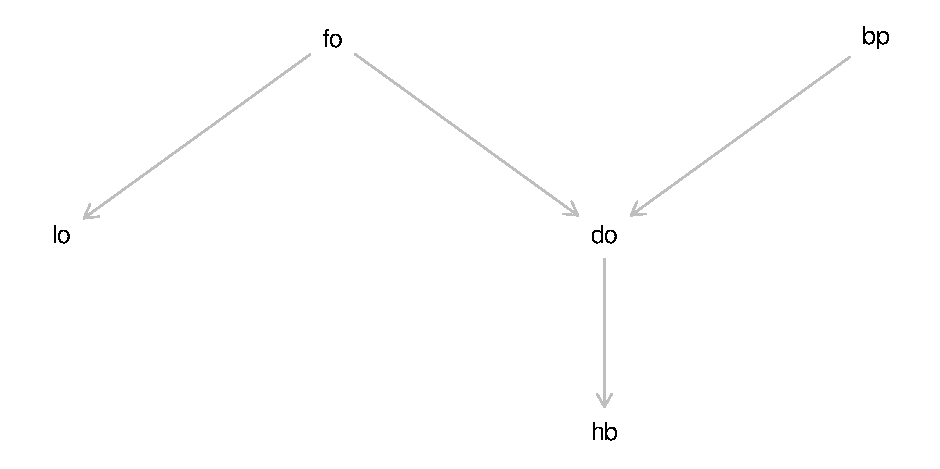
\includegraphics[scale=0.6]{pics/fodagitty.pdf}
	\end{figure} 





 
\end{itemize}



} 

\end{frame}


\begin{frame}{The Family Out Problem}
\scriptsize{



\begin{itemize}
\item Let's try to understand now the built-in independence assumptions of this DAG.

\item Consider the random variables family-out $fo$ and hear-bark $hb$.

\item Are these variables independent? 

\item Intuitively not, because if his family leaves home, then the dog is more likely to be out.
\item Thus, he is more likely to hear it bark. 

\item However, what if he knows that dog-out $do$ is true or false?

\item Now $hb$ is independent of $fo$ given $do$, $f(hb | fo, do) = f(hb | do)$.

\item Hearing the dog bark was dependent on her being in or out.

\item Once he knows whether she is in or out, then where the family is is of no concern.





 
\end{itemize}



} 

\end{frame}


\begin{frame}{The Family Out Problem}
\scriptsize{



\begin{itemize}
\item Note that if we wanted to say that the location of the family is directly relevant to hearing the dog bark, then we would have to put another arc directly between the two variables.
\item Direct relevance would occur, say, if the dog is more likely to bark when the family is away than when it is at home.
\item This is not the case here.

\item Now we can give the rule specifying dependence and independence in DAGs.

\item In a DAG, a variable $A$ is dependent on a variable $B$ given evidence $E=\{E_1,\dots,E_m\}$ if there is a d-connecting path from $A$ to $B$ given $E$.

 
\end{itemize}



} 

\end{frame}


\begin{frame}{D-separation}
\scriptsize{
\begin{itemize}

\item We need to keep in mind that there are only four types of variable relations that combine to form all possible undirected paths in a DAG \cite{mcelreath2020statistical}.

\item For a random variable $Z$ and its two immediate neighbors in the path $X$ and $Y$, the 4 possible relations are:

  \begin{figure}[h!]
	\centering
	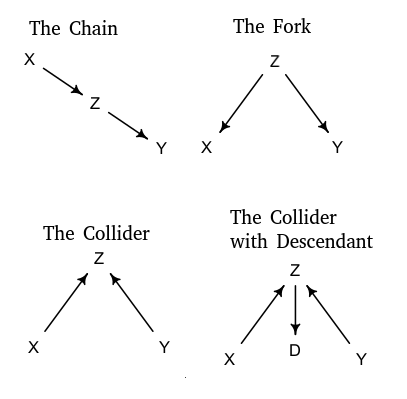
\includegraphics[scale=0.61]{pics/collider.png}
	\end{figure} 


 
 
\end{itemize}



} 

\end{frame}



\begin{frame}{D-separation}

\begin{block}{Definition}
 \begin{itemize}

\item An undirected path from $A$ to $B$ is d-connecting with respect to the evidence nodes $E$ if \textbf{every} interior node $E_i$ in the path satisfies one of these two rules:

\begin{enumerate}
 \item It is a chain or a fork and not a member of E.
 \item It is a collider, and either $E_i$ or one of its descendants is in E.
\end{enumerate}
 
 
\end{itemize}

\end{block}



\begin{itemize}


\item In the literature, the term d-separation is more common.

\item Two nodes are d-separated if there is no d-connecting path between them.


\item So, if $A$ and $B$ are d-separated given $E$, they are conditionally independent $A \perp B |E$. 

 
 
\end{itemize}





\end{frame}



\begin{frame}[fragile]{Rule 1}
\scriptsize{
\begin{itemize}

\item The rule 1 tells us that a d-connecting path must not be \textbf{blocked} by evidence.

\item This means that once we know about a middle node, we do not need to know about anything further away.

\item For example, the path from $fo$ to $hb$, $fo \rightarrow do \rightarrow hb$ forms a chain.

\item We already discussed that $fo$ and $hb$ are dependent from each other, but conditionally independent given $do$.

\item Now we can use the first rule of d-separation to answer these questions about dependency.

\item Let's use the commands \textbf{dconnected} and \textbf{dseparated} from daggity.

\begin{verbatim}
> dconnected(fo,"fo","hb",c()) 
[1] TRUE
> dseparated(fo,"fo","hb",c()) 
[1] FALSE
> dconnected(fo,"fo","hb",c("do")) 
[1] FALSE
> dseparated(fo,"fo","hb",c("do")) 
[1] TRUE
\end{verbatim}

\item So, $do$ blocks the path between $fo$ and $hb$.




\end{itemize}

} 

\end{frame}


\begin{frame}[fragile]{Rule 1}
\scriptsize{
\begin{itemize}

\item Let's consider the path with a fork: $lo \leftarrow fo \rightarrow do$.

\item By rule 1, $lo$ and $do$ are d-connected but d-separated give $fo$.

\begin{verbatim}
> dconnected(fo,"lo","do",c()) 
[1] TRUE
> dconnected(fo,"lo","do",c("fo")) 
[1] FALSE
\end{verbatim}


\item So $fo$ blocks the path between $lo$ and $do$.

\item From a causal point of view, this is the classical problem of confounding.

\item Light-on and dog-out are both caused by family-out, hence they are dependent.

\item However, once the cause if known, they become independent.





\end{itemize}

} 

\end{frame}


\begin{frame}[fragile]{Rule 1}
\scriptsize{
\begin{itemize}

\item Rule 1 also tell us that there can be no colliding interior nodes in the path.

\item Let's consider the path from $fo$ to $bp$, $fo \rightarrow do \leftarrow bo$.

\item Here we have a collider (not a fork nor a chain), so by rule one $fo$ and $bp$ are marginally independent.

\begin{verbatim}
> dconnected(fo,"fo","bp",c())
[1] FALSE 
\end{verbatim}



\item If two things can cause the same state of affairs and have no other connections, then the two things are independent.




\end{itemize}

} 

\end{frame}


\begin{frame}[fragile]{Rule 2}
\scriptsize{
\begin{itemize}

\item Suppose we know that the dog is out (i.e., dog-out is a member of $E$)

\item Now, are family-out and bowel-problem conditionally independent given dog-out?

\item By rule number 2 we know that fo and bp given do are d-connected (a collider node in the evidence).

\begin{verbatim}
> dconnected(fo,"fo","bp",c("do"))
[1] TRUE 
\end{verbatim}

\item So, they became dependent given the evidence.

\item How do we explain this?

\item For example, if we know that the dog is out, knowing that the family is at home should raise (slightly) the probability that the dog has bowel problems.

\item Because we eliminated the most likely explanation for the dog being out, less likely explanations become more likely.

\end{itemize}

} 

\end{frame}


\begin{frame}[fragile]{Rule 2}
\scriptsize{
\begin{itemize}

\item We would have a similar situation if we did not know that the
dog was out but heard the barking.

\item Since $hb$ is a descendant of the collider node $do$, $fo$ and $bp$ are d-connected with respect to $hb$:

\begin{verbatim}
> dconnected(fo,"fo","bp",c("hb"))
[1] TRUE 
\end{verbatim}



\item In this case, we would not be sure the dog was out, but we do have relevant evidence (which raises the probability), so hear-bark, in effect, connects the two nodes above the collider. 

\item Intuitively, rule 2 means that a d-connecting path can only go through a collider if we are conditioning on any of its potential effects.

\item By ``any effect'' we mean the collider node itself or any of its descendants.
\end{itemize}

} 

\end{frame}


\begin{frame}[fragile]{Rule 2}
\scriptsize{
\begin{itemize}

\item We have finished the explanation of d-separation.

\item This is undoubtedly the most difficult part of DAGs to understand.

\item Exercise: explain all the conditional independencies of the family out DAG using the rules of d-separation.

\begin{verbatim}
> impliedConditionalIndependencies(fo)
bp _||_ fo
bp _||_ hb | do
bp _||_ lo
do _||_ lo | fo
fo _||_ hb | do
hb _||_ lo | fo
hb _||_ lo | do 
\end{verbatim}




\end{itemize}

} 

\end{frame}



\begin{frame}{Causal DAGs}
\scriptsize{
\begin{itemize}


\item The interpretation of DAGs as carriers of independence assumptions does not necessarily imply \textbf{causation}.

\item For example, for a DAG consisting only of chains, we could reverse the order of all the arrows while retaining all the encoded independence assumptions.

\item From a causal point of view, such a change would completely change the causal order of things.

\item \textbf{Causal inference} is a huge topic and goes beyond the scope of this course.

\item When DAGs are given a causal interpretation, they are usually called \textbf{causal graphs} or \textbf{causal diagrams}.


\item This causal interpretation allows us to infer causes from observed effects (if the light is on and the dog is out, then his family is probably out).

\item It is this causal interpretation that explains why DAG models are rarely used in any variable ordering other than those which respect the direction of \textbf{time} and \textbf{causation}. \cite{pearl2009causality}

\end{itemize}



} 

\end{frame}




\begin{frame}{Causal Inference}


\begin{figure}[h!]
	\centering
	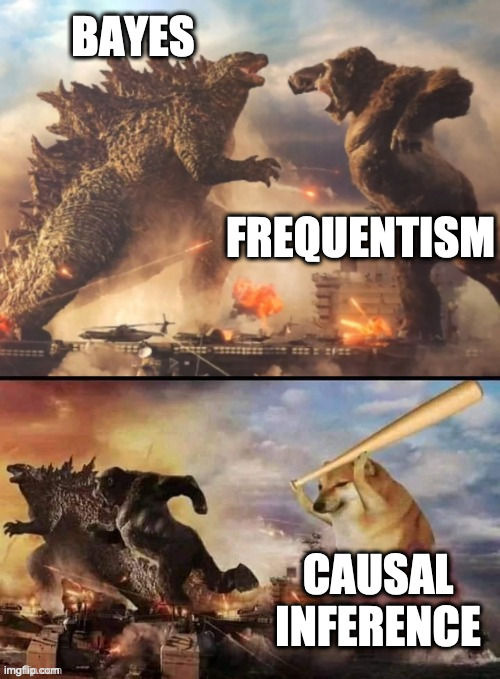
\includegraphics[scale=0.3]{pics/causalMeme.jpeg}
	\end{figure} 



\end{frame}


\begin{frame}{Causal Inference}
\scriptsize{
\begin{itemize}


\item DGMs or Bayesian Networks are very fundamental in causal inference.

\item Judea Pearl, the creator of them is also a foundational figure in causal inference.

\item His book, ``The Book of Why'' \cite{pearl2018book} is a highly recommended introduction to the field.

\end{itemize}


\begin{figure}[h!]
	\centering
	
\includegraphics[scale=0.3]{pics/bookofwhy.png}
	\end{figure} 




} 

\end{frame}



\begin{frame}{Estimation for DAGs}
\scriptsize{
\begin{itemize}
\item Two estimation questions arise in the context of DAGs. 
\item First, given a DAG $\mathcal{G}$ and data $d_1,\dots,d_n$ from a distribution $f$ consistent with $\mathcal{G}$, how do we estimate f?

\item Second, given data $d_1,\dots,d_n$ how do we estimate $\mathcal{G}$?

\item The first question is pure estimation while the second involves model selection.

\item These are very involved topics and are beyond the scope of this course.

\item We will just briefly mention the main ideas.

 
\end{itemize}



} 

\end{frame}


\begin{frame}{Estimation for DAGs}
\scriptsize{
\begin{itemize}

\item If we are doing frequentist inference, we typically use some parametric model $f(x|\pi_x;\theta_x)$ for each conditional density. 

\item The likelihood function is then

\begin{displaymath}
 \mathcal{L}(\theta) = \prod_{i=1}^nf(d_i;\theta) ) =  \prod_{i=1}^n\prod_{j=1}^mf(X_{ij}|\pi_j;\theta_j) 
\end{displaymath}

\item where $X_{ij}$ is the value of $X_j$ for the ith data point and j are the parameters for the-jth conditional density. 

\item We can then estimate the parameters by maximum likelihood.

\item On the other hand, if we want to perform Bayesian inference we must set priors for all our variables $X_1,\dots,X_m$ and estimate the posterior accordingly (using MCMC for example).

 
\end{itemize}



} 

\end{frame}

\begin{frame}{Estimation for DAGs}
\scriptsize{
\begin{itemize}

\item To estimate the structure of the DAG itself, we could fit every possible DAG using maximum likelihood and use AIC (or some other method) to choose a DAG. 

\item However, there are many possible DAGs so we would need much data
for such a method to be reliable.

\item Also, searching through all possible DAGs is a serious computational challenge. 

\item Producing a valid, accurate confidence set for the DAG structure would require astronomical sample sizes. 

\item If prior information is available about part of the DAG structure, the computational and statistical problems are at least partly ameliorated \cite{wasserman2013all}.

 
\end{itemize}



} 

\end{frame}


\begin{frame}{Plate Notation}
\scriptsize{
\begin{itemize}
\item DGM are widely used to represent probabilistic machine learning models.

\item For example: Naive Bayes, Latent Dirichlet Allocation, Hidden Markov Models.

\item However, when the number of variables is large, the standard DAG notation is not useful.

\item Plate notation is a method of representing variables that repeat in a DAG.

\item A plate or rectangle is used to group variables into a subgraph that repeat together.

\item A number is drawn on the plate to represent the number of repetitions of the subgraph in the plate.
 
\end{itemize}



} 

\end{frame}

\begin{frame}{Plate Notation}
\scriptsize{


\begin{figure}[h!]
	\centering
	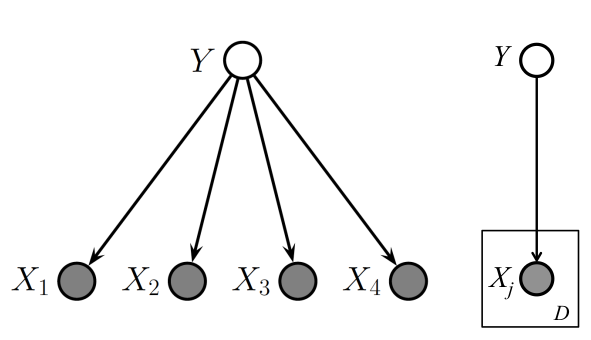
\includegraphics[scale=0.35]{pics/plate.png}
	\end{figure} 


\begin{itemize}
\item Left: variables $X_j$ are conditionally independent given $Y$. 
\item Right: Same model, using plate notation. 
\item This represents the same model as the one on the left, except the repeated $X_j$ nodes are inside a box, known as a plate.
\item The number in the lower right hand corner, $D=4$ , specifies the number of repetitions of the $X_j$ node. 
\item  Shaded nodes indicate observed data. 
\item Open nodes are latent/hidden (e.g., a parameter in Bayesian inference).

\end{itemize}



} 

\end{frame}



\begin{frame}{A real-world application}
\scriptsize{
\begin{itemize}
\item  The Netherlands Forensic Institute uses the  \textbf{Bonaparte DNA-matching software}  every day, mostly for missing-persons cases, criminal investigations, and immigration cases \cite{pearl2018book}. 


\item Applicants for asylum must prove that they have fifteen family members in the Netherlands.

 \item The idea behind Bonaparte is to make it possible to use DNA information from more distant relatives or from multiple relatives.

  
\item Bonaparte does this by converting the pedigree of the family  into a DAG.

\item The central problem is that the genotype of an individual, detected in a DNA test, contains a contribution from both the father and the mother, but we cannot tell which part is which.


\item Thus these two contributions (called ``alleles'') have to be treated as hidden, unmeasurable variables in the Bayesian network.




 
\end{itemize}



} 

\end{frame}


\begin{frame}{A real-world application}

\begin{figure}[h!]
	\centering
	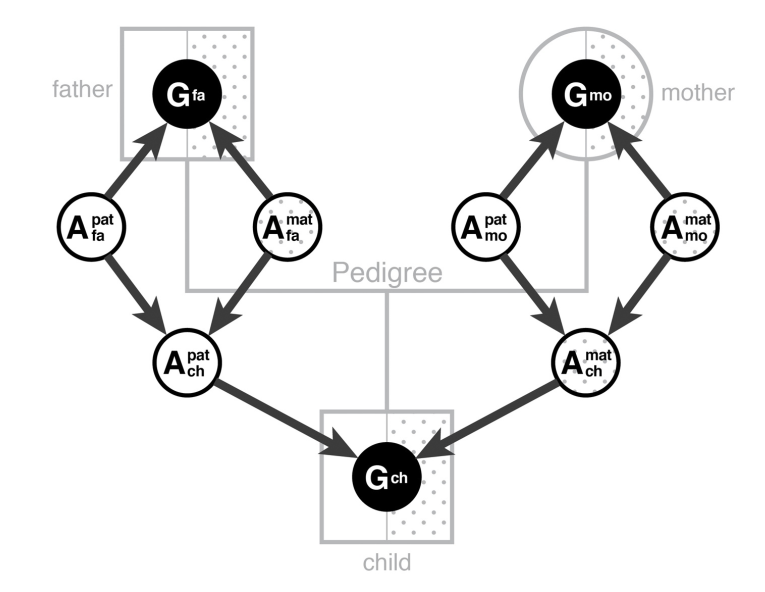
\includegraphics[scale=0.3]{pics/bonaparte.png}
	\caption{The figure shows  how Bonaparte converts one small piece of a pedigree to a (causal) DAG \cite{pearl2018book}}
	\end{figure} 


\end{frame}



\begin{frame}{A real-world application}
\scriptsize{
\begin{itemize}

\item The system did it most impressive work after a massive disaster, such as the crash of Malaysia Airlines Flight 17.

\item Few, if any, of the victims of the plane crash could be identified by comparing DNA from the wreckage to DNA in a central database. 

\item The next best thing to do was to ask family members to provide DNA swabs and look for partial matches to the DNA of the victims.

\item Part of Bonaparte's job is to infer the probability of the cause from the evidence. 

\item Cause example: the victim's gene for blue eyes came from his father.

\item Evidence examples: he has a blue-eyed gene and a black-eyed gene, his cousins on the father's side have blue eyes, but his cousins on the mother’s side have black eyes. 
 
\end{itemize}



} 

\end{frame}



\begin{frame}{A real-world application}

\begin{figure}[h!]
	\centering
	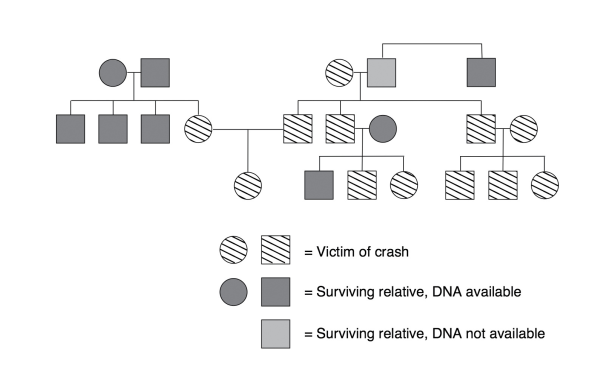
\includegraphics[scale=0.45]{pics/malasyia.png}
	\caption{Actual pedigree of a family with multiple victims in the Malaysia Airlines crash \cite{pearl2018book}}
	\end{figure} 

\end{frame}

\begin{frame}{A real-world application}
\scriptsize{
\begin{itemize}

\item Once the DAG is set up, the final step is to input the victim's
DNA and compute the likelihood that it fits into a specific slot in the pedigree.

\item This is done by belief propagation with Bayes’s rule.

\item The DAG begins with a particular degree of belief in each possible statement about the nodes in the network, such as ``this person's paternal allele for eye color is blue.'' 
\item As new evidence is entered into the network—at any place in the network—the degrees of belief at every node, up and down the network, will change in a cascading fashion. 
\item Thus, for example, once we find out that a given sample is
a likely match for one person in the pedigree, we can propagate that
information up and down the network. 
\item In this way, Bonaparte not only learns from the living family members' DNA but also from the identifications it has already made.
\end{itemize}



} 

\end{frame}




\begin{frame}{Conclusions}
\scriptsize{

\begin{itemize}
\item This class introduced Directed Graphical Models (aka Bayesian Networks), a probabilistic framework for encoding conditional independence relation using graphs.

\item We have introduced the three main mathematical ideas behind them: conditional independence, the chain rule of probability, and DAGs.

\item D-separation is a rule for establishing whether two variables are conditionally independent given another in a DAG.

\item DAGs play an important role in both machine learning and causal inference.



\end{itemize}


} 
\end{frame}


%%%%%%%%%%%%%%%%%%%%%%%%%%%
\begin{frame}[allowframebreaks]\scriptsize
\frametitle{References}
\bibliography{bio}
\bibliographystyle{apalike}
%\bibliographystyle{flexbib}
\end{frame}  









%%%%%%%%%%%%%%%%%%%%%%%%%%%

\end{document}
